\documentclass[a4paper, 10pt]{article}
\usepackage[english]{babel}
\usepackage[utf8]{inputenc}
\usepackage{amsmath}
\usepackage{graphicx}
\usepackage{float}
\usepackage{fixltx2e}
\usepackage{listings}
\usepackage{color}
\usepackage{latexsym}
\usepackage{lstautogobble}
\usepackage[colorinlistoftodos]{todonotes}
\usepackage[margin=3cm]{geometry}
\usepackage{hyperref}
\usepackage{tikz}
\hypersetup{
	hidelinks, 
	colorlinks = true,
	linkcolor = black,
}

\usetikzlibrary{shapes, arrows}

\newtheorem{definit}{Definizione}[subsection]
\newcommand{\encr}{E_e}
\newcommand{\decr}{D_d}
\newcommand{\pua}{PU_a}
\newcommand{\pub}{PU_b}
\newcommand{\pra}{PR_a}
\newcommand{\prb}{PR_b}

\begin{document}
	\clearpage
	\begin{titlepage}
		\centering
		\vspace*{\fill}
		{\scshape\LARGE Università degli Studi di Verona \par}
		\vspace{1.5cm}
		\line(1,0){230} \\
		{\huge\bfseries Sicurezza delle reti\par}
		\line(1,0){230} \\
		\vspace{0.5cm}
		{\scshape\Large Riassunto dei principali argomenti\par}
		\vspace{2cm}
		{\Large\itshape Davide Bianchi\par}
		\vspace{1cm}
		\vspace{5cm}
		\vspace*{\fill}
		% Bottom of the page
		{\large \today\par}
	\end{titlepage}
	\thispagestyle{empty}
	\newpage
	\tableofcontents
	\newpage
	
	\section{Introduzione}
	
	\begin{definit}[Information Security]
		Protezione delle informazioni e dei sistemi per impedirne l'accesso non autorizzato, uso, divulgazione, modifica o distruzione.
	\end{definit}
	
	\begin{definit}[Network Security]
		Protezione dell'accesso a risorse situate all'interno di una rete.
	\end{definit}
	
	Nella sicurezza si distinguono una \textbf{policy}, un \textbf{meccanismo} e una \textbf{compliance}.
	Una security policy specifica il comportamento che il sistema può o non può assumere. I meccanismi di sicurezza sono l'implementazione di una data policy. Diciamo quindi che una security policy $\phi$ deve rimanere valida per un sistema $P$ in ogni ambiente malevolo $E$, ovvero $P \parallel E \models \phi $.
	
	Le politiche di sicurezza sono spesso formulate per arrivare ad alcune proprietà standard, le più comuni sono:\begin{itemize}
		\item Confidenzialità: non ci sono fughe di informazioni;
		\item Integrità: non ci sono modifiche alle informazioni;
		\item Disponibilità: non ci sono "danneggiamenti" ai servizi;
		\item Accountability\footnote{La traduzione più vicina è \textit{responsabilità}.}: le azioni sono sempre riconducibili ai diretti responsabili;
		\item Autenticazione: l'origine dei dati può essere identificata con sicurezza.
	\end{itemize}
	
	\paragraph{Contromisure per la protezione.} Le principali tecniche di contromisura consistono in:\begin{itemize}
		\item Prevenzione di breach;
		\item Rilevamento di attacchi in corso;
		\item Reazione ad un possibile attacco.
		\end{itemize}
		
	\section{Cenni di crittografia}
	\subsection{Introduzione}
	Iniziamo dando alcune definizioni fondamentali. Si useranno i termini \textit{ciphertext} e \textit{plaintext} per indicare rispettivamente il testo cifrato e quello in chiaro.
	
	\begin{definit}[Crittografia]
	Insieme dei metodi per rendere un messaggio non leggibile ad altri.
	\end{definit}
	
	\begin{definit}[Steganografia]
	Insieme dei metodi per nascondere l'esistenza di un messaggio in un altro contenuto.
	\end{definit}
	
	\begin{definit}[Crittoanalisi]
	Analisi del ciphertext per ottenere il plaintext corrispondente.
	\end{definit}
					
	Un generico sistema crittografico è strutturato come: \\
	
	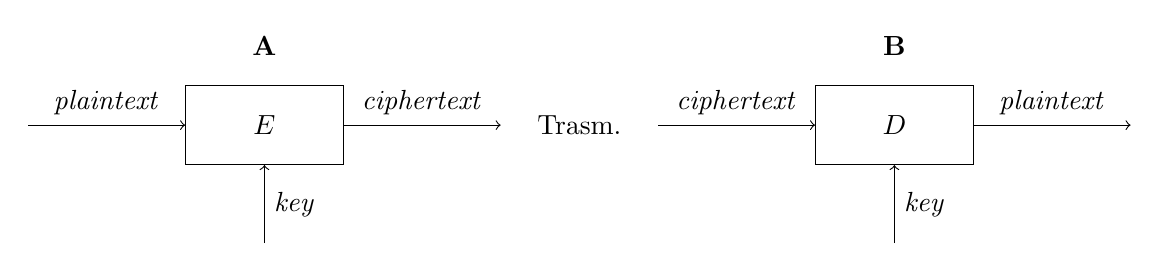
\begin{tikzpicture}
	\node at (4,0) [rectangle,draw, minimum width=2cm, minimum height=1cm] (E) {$E$};
	\draw (E);
	\draw[->] (1,0) -- (E) node[above, midway] {\textit{plaintext}};
	\draw[->] (4,-1.5) -- (E) node[right, midway] {\textit{key}};
	\draw[->] (E) -- (7,0) node[above, midway] {\textit{ciphertext}};
	\node at (8,0) (dots) {Trasm.};
	\node at (12,0) [rectangle,draw, minimum width=2cm, minimum height=1cm] (D) {$D$};
	\draw[->] (9,0) -- (D) node[above, midway] {\textit{ciphertext}};
	\draw[->] (12,-1.5) -- (D) node[right, midway] {\textit{key}};
	\draw[->] (D) -- (15,0) node[above, midway] {\textit{plaintext}};
	\node at (4,1) {\textbf{A}};
	\node at (12,1) {\textbf{B}};
	\end{tikzpicture}
	
	In crittografia si distinguono le due categorie \textit{a chiave simmetrica} e \textit{a chiave asimmetrica}. La differenza sta nel fatto che nella crittografia a chiave simmetrica le due entità che si scambiano il messaggio devono condividere una stessa chiave (che deve essere trasmessa su un canale sicuro), mentre nella crittografia a chiave asimmetrica le chiavi sono differenti e sono 2 per ogni entità, una pubblica e una privata. Nella crittografia a chiave asimmetrica si elimina il problema della condivisione della chiave; inoltre la chiave pubblica può essere compromessa da attaccanti senza che la chiave privata venga compromessa, e senza che venga compromessa la segretezza del messaggio.
	
	Un altro aspetto fondamentale della crittografia è che la cifratura e la decodifica sono facili, \textit{se le chiavi sono note}. Da ciò consegue che la sicurezza debba risiedere nella chiave, non nell'algoritmo in se.
	
	\subsection{Crittoanalisi}
	La scienza di recuperare il messaggio in chiaro senza conoscere il ciphertext si basa sostanzialmente su due differenti approcci:
	\begin{itemize}
		\item attacco brute-force;
		\item attacco crittoanalitico.
	\end{itemize}
	
	\paragraph{Attacco brute-force.} Un attacco bruteforce è semplice: consiste nel provare tutte le chavi possibili fino ad indovinare quella corretta. Questa tipologia di attacco in generale è sempre possibile nella sua semplicità, tuttavia, se la dimensione dello spazio delle chiavi inizia ad essere elevata, il tempo che si deve impiegare diventa insostenibile, per cui in questi casi è necessario ricorrere ad altri stratagemmi.
	
	\paragraph{Attacco crittoanalitico.} In questo caso si assume che l'attaccante conosca l'algoritmo utilizzato nella cifratura dei messaggi; si trova quindi una qualche debolezza nell'algoritmo che permetta di farlo fallire. 
	
	In tal senso, si tende a rendere noto un algoritmo affinchè il maggior numero di persone tenti di attaccarlo, per aumentare al massimo le possibilità che venga trovata una falla. (In contrasto con la cosiddetta \textbf{security by obscurity}).
	
	\paragraph{Tipologie di attacco.}Consideriamo ora i possibili attacchi che un sistema crittografico deve affrontare per essere affidabile:
	\begin{itemize}
		\item \textit{known cypertext attack:} questo attaccante è il meno aggressivo e conosce solamente il testo cifrato;
		
		\item \textit{known plaintext attack:} conosce entrambi i tipi di testo;
		
		\item \textit{choosen plaintext:} può scegliere il plaintext da codificare e analizzare il ciphertext ottenuto;
		
		\item \textit{adaptive choosen plaintext:} può liberamente scegliere il plaintext da far codificare e comportarsi di conseguenza, sulla base del risultato appena ottenuto.
		
		\item \textit{chosen ciphertext:} l'attaccante può scegliere differenti ciphertext e avere accesso al plaintext decriptato, per infine ricavare la chiave.
		\end{itemize}
	
	\subsection{Notazione} \label{notation}
	La notazione usata è la seguente: \begin{itemize}
		\item $\mathcal{A}$ è l'alfabeto, ovvero un insieme finito di simboli;
		\item $\mathcal{M} \subseteq \mathcal{A}^*\star$ è il messaggio, dove $M \in \mathcal{M}$ è il \textit{plaintext};
		\item $\mathcal{C}$ è il messaggio cifrato, il cui alfabeto può anche differire da quello usato per $M$;
		\item $\mathcal{K}$ indica lo spazio delle chiavi;
		\item ogni $e \in \mathcal{K}$ denota una funzione biiettiva da $\mathcal{M}$ a $\mathcal{C}$, viene indicata con $\encr$ ed è la funzione di cifratura;
		\item ogni $d \in \mathcal{K}$ è una funzione biiettiva da $\mathcal{C}$ a $\mathcal{M}$, indicata con $\decr$ ed è la funzione di decodifica.
	\end{itemize}

	Data la notazione soprastante, indichiamo con cifrario un insieme $\lbrace \encr\ |\ e \in \mathcal{K} \rbrace$ e il suo corrispondente $\lbrace \decr\ |\ d \in \mathcal{K} \rbrace$ tale che per ogni $e \in \mathcal{K}$ esiste un solo $d \in \mathcal{K}$, in modo tale che $\decr = \encr^{-1}$. La coppia $\langle e, d \rangle$ forma una coppia di chiavi, dove $e$ e $d$ possono anche essere identiche (come nel caso della crittografia simmetrica).
	
	\section{Crittografia a chiave simmetrica}
	Nella crittografia a chiave simmetrica le chiavi sono le stesse ($e = d$), e i due interlocutori condividono una chiave. I cifrari possibili nel caso della crittografia simmetrica sono di 3 categorie: \begin{itemize}
		\item \textit{cifrari a blocchi:} dividono il testo in blocchi di lunghezza fissa e cifrano un blocco alla volta;
		\item \textit{cifrari a flusso:} cifrari a blocchi in cui la dimensione di ogni blocco è fissata a 1;
		\item \textit{codes:} cifrari che lavorano su parole a lunghezza variabile.
	\end{itemize}

	\subsection{Tecniche di sostituzione}
	Sono tutti quei cifrari che sostituiscono una lettera con un'altra lettere, basandosi su una qualche regola di sostituzione, come il cifrario di Cesare e la permutazione casuale.
	
	\paragraph{Cifrario di Cesare.}
	Il messaggio viene cifrato sostituendo ogni lettera $l$ del messaggio con la $l+k$ esima lettera dell'alfabeto; la chiave quindi è data dalla coppia $(l, l+k)$. 
	
	Il cifrario di Cesare è facile da attaccare in quanto basta un attacco \textit{bruteforce}, quindi è sufficiente provare tutte le combinazioni (che sono in totale 26).
	
	\paragraph{Permutazione casuale.}
	Supponiamo di usare come cifrario una permutazione casuale dell'alfabeto, ovvero sostituendo ad ogni lettera dell'alfabeto un'altra lettera, in modo totalmente casuale. In tal caso l'attacco bruteforce richiederebbe tempo eccessivo (ci sono $26!$ pssibili combinazioni da provare, che sono decisamente troppe). 
	
	La tecnica usata per attaccare questo tipo di crittografia è l'\textit{analisi delle frequenze}, ovvero l'analisi delle lettere che capitano di più in una data lingua, e associare la lettera del messaggio cifrato con una data frequenza con quella nella lingua del messaggio con una frequenza simile.
	
	\paragraph{Cifrario di Vigenère.}
	Il cifrario di Vigenère riprende l'idea del cifrario di Cesare. L'idea è la seguente: presa una chiave (es. \textit{key}), si ripete la chiave tante volte quanto è lungo il testo (eventualmente troncando l'ultima ripetizione), e si codifica la lettera con il corrispondete cifrario di Cesare. \\
	
	\noindent
	K E Y K E Y K E Y K E Y \\
	P R O V A D I T E S T O \\
	
	
	La prima lettera del cipher text sarà la lettera ottenuta dal cifrario di Cesare di chiave $(K,P)$, la seconda con la chiave $(E, R)$ e così via.
	
	Anche questo cifrario è semplice da attaccare, si parte dalla divisione del ciphertext in gruppi di lunghezza pari a quella della chiave, e si esegue l'analisi delle frequenze su ogni gruppo.
	
	\subsection{Cifrari a trasposizione}
	Funzionano in maniera leggermente diversa. Dato un blocco di lunghezza $l$ e $\mathcal{K}$ un insieme di permutazioni su $\lbrace 1 \dots t \rbrace$, si ha che \[ \encr(m) = m_{e(1)}, \dots, m_{e(2)} \] Per decodificare si applica la permutazione inversa ad ogni carattere del ciphertext.
	
	\subsection{Cifrario di Feistel}
	
	\subsection{Data Encryption Standard (DES)}
	È un cifrario a blocchi che lavora su blocchi di 64 bit. Fu in effetti il primo standard di crittografia, e ne furono rilasciate versioni aggiornate che lavorassero su chiavi di lunghezza maggiore (3-DES). Non è ancora stato violato, ma è possibile ridurre in tempo lineare lo spazio delle chiavi da $2^{56}$ a $2^{43}$.
	
	\begin{center}
		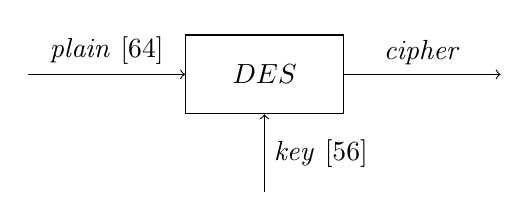
\begin{tikzpicture}
		\node at (4,0) [rectangle,draw, minimum width=2cm, minimum height=1cm] (E) {$DES$};
		\draw (E);
		\draw[->] (1,0) -- (E) node[above, midway] {\textit{plain} $\left[ 64 \right]$};
		\draw[->] (4,-1.5) -- (E) node[right, midway] {\textit{key} $\left[ 56 \right]$};
		\draw[->] (E) -- (7,0) node[above, midway] {\textit{cipher}};
		\end{tikzpicture}
	\end{center}
	
	\subsubsection{Double DES e 3-DES}
	La variante DD, che usa DES due volte consecutive, è soggetta ad un attacco del tipo \textit{Meet-in-the-Middle}.
	\begin{center}
		\begin{tikzpicture}
		\node at (4,0) [rectangle,draw, minimum width=2cm, minimum height=1cm] (E) {$DES$};
		\draw (E);
		\draw[->] (1,0) -- (E) node[above, midway] { $P_1$};
		\draw[->] (4,-1.5) -- (E) node[right, midway] {$K_1$};
		\draw[->] (E) -- (7,0) node[above, midway] {$M$};
		\node at (8,0) [rectangle,draw, minimum width=2cm, minimum height=1cm] (2E) {$DES$};
		\draw[->] (8,-1.5) -- (2E) node[right, midway] {$K_2$};
		\draw[->] (2E) -- (11,0) node[above, midway] { $P_2$};
		\end{tikzpicture}
	\end{center}

	L'attacco funziona nel seguente modo: \begin{enumerate}
		\item Dato un $C = E_{K_2}(E_{K_1}(P))$, sia $X = E_{K_1}(P) = D_{K_2}(C)$;
		\item Dati $P$ e $C$, cifrare $P$ per ogni possibile chiave (sono $2^{56}$);
		\item Generare una tabella con tutti i risultati, ordinati secondo $X$;
		\item Decifrare $C$ con tutte le possibili $K_2$, cercando un matching con quelle i risultati ottenuti prima. Ogni coppia è una possibile coppia valida, basta confrontare i risultati con $P$ e $C$ iniziali.
	\end{enumerate}

	In effetti, guardando lo schema sopra, si nota che al massimo occorrono $2^{56}$ operazioni per violare questo protocollo.
	
	Con 3-DES invece, un tentativo con la soluzione bruteforce necessita di almeno $2^{112}$ operazioni, un numero notevolmente più alto. Al momento infatti non esistono soluzioni per violare 3-DES.
	
	\subsection{Advanced Encryption Standard (AES)}
	Proposto come rimpiazzo di DES nel 1991, fu selezionato nel 2001. Infatti il DES iniziava a non andare più bene, in larga parte perchè era disegnato per i software degli anni 70 ed era abbastanza lento. AES funziona in maniera più snella e lavora su chiavi molto più lunghe (128, 192 e 256 bit).
	
	\subsection{Cipher block chaining}
	Come ci si comporta quando la lunghezza del messaggio eccede la dimensione del blocco? In tal caso, ci sono molteplici possibilità:\begin{enumerate}
		\item Splittare il messaggio in $m$ blocchi, e cifrarli individualmente. Questa opzione è soggetta a pesanti limtazioni, la prima data dal fatto che identici plaintext vengono mappati su identici ciphertext (\textit{information leak}); la seconda invece limita di parecchio le possibilità di individuare eventuali manomissioni del messaggio da parte di terzi (\textit{integrity});
		
		\item Si può pensare in alternativa di far dipendere un carattere del ciphertext da quello precedente: dato un valore iniziale, il successivo carattere sarà cifrato con uno XOR tra il carattere precedentemente cifrato e il carattere da cifrare. In sostanza, dato un certo $C_0$, \begin{align*}
			C_i &= E_K(P_i \oplus C_{i-1}) \\
			P_i &= C_{i-1} \oplus D_K(C_i) \quad \text{(per la decodifica)}
		\end{align*}
	\end{enumerate}

	Con la seconda soluzione, i caratteri cifrati dipendono strettamente da quelli precedenti, quindi è impossibile che due plaintext uguali vengano mappati su ciphertext uguali.
	
	\subsection{Posizionamento dei sistemi crittografici}
	Distinguiamo i casi di \textit{link encryption} e \textit{end-to-end encryption}.
	Nella link encryption ci sono sistemi di cifratura ad ogni collegamento, quindi i dati vengono decifrati e cifrati ad ognuno dei singoli collegamenti. Nella crittografia end-to-end invece, ciò che accade è che i sistemi di cifratura sono posizionati all'origine e alla destinazione dei dati, però in tal caso è necessario l'utilizzo di chiavi condivise tra i due interlocutori.
	
	Guardando la questione da un punto di vista alternativo, ossia quello dello stack OSI, possiamo osservare come la link encryption sia applicata ai livelli più bassi dello stack, mentre man mano si sale viene applicata una crittografia di tipo end-to-end. Idealmente, serve che la crittografia end-to-end protegga i dati contenuti nei pacchetti, ma che lasci inalterati gli header, per permettere l'inoltro dei pacchetti. La link encryption protegge invece i dati di inoltro da monitoraggio e analisi da parte di terzi.
	
	\subsection{Distribuzione delle chiavi}
	Come già detto in precedenza, la crittografia a chiave simmetrica richiede che le parti condividano una chiave. Ciò può costituire un problema, dal momento che terzi malintenzionati possono sempre tentare di rubare la chiave sfruttando qualche falla nel sistema di condivisione della stessa.
	
	Tipicamente non viene usata una sola chiave, ma una gerarchia di chiavi. Si ha quindi:\begin{itemize}
		\item \textit{session key:} usata per crittografare dati per una sola sessione logica;
		\item \textit{master key:} usata per cifrare le sessioni.
	\end{itemize}

	I problemi principali che si possono incontrare quindi sono i seguenti: \begin{itemize}
		\item la gerarchia delle chiavi è necessaria per reti molto vaste, ma è necessaria una sorta di garanzia sulle chiavi;
		
		\item il tempo di vita della chiave di sessione deve essere il minore possibile;
		
		\item l'uso di un sistema automatico di ditribuzione delle chiavi necessita la fiducia da parte degli utenti;
		
		\item il sistema di distribuzione è decentralizzato;
		
		\item è necessario stabilire una politica di controllo sull'uso delle chiavi.
	\end{itemize}

	\section{Crittografia a chiave pubblica}
	\paragraph{Notazione.} Oltre alla notazione specificata nella sezione \ref{notation}, specifichiamo con $PU_b$ e $PR_b$ rispettivamente la chiave pubblica di B e la chiave privata di B.
	
	\subsection{Struttura del sistema}
	Questo tipo di crittografia elimina il problema della distribuzione delle chiavi, in quanto ogni utente ha due chiavi, una pubblica (che tutti possono vedere), e una privata (che \textit{dovrebbe} rimanere incognita).
	
	Ogni utente genera una coppia di chiavi, una pubblica e una privata. Quella pubblica viene inserita in un registro.
	Supponiamo che B voglia inviare un messaggio ad A. La procedura è la seguente:\begin{enumerate}
		\item B cifra il messaggio con la chiave pubblica di A;
		\item A riceve il messaggio cifrato trasmesso da B;
		\item A decifra il messaggio ricevuto usando la sua chiave privata.
	\end{enumerate}

	\subsection{Crittoanalisi della crittografia a chiave pubblica}
	Gli attacchi possibili sono i seguenti: \begin{itemize}
		\item \textit{Bruteforce:} l'unica soluzione è aumentare la lunghezza della chiave, cosa che potrebbe non scalare bene con l'aumentare della dimensione, data la complessità dell'algoritmo; in pratica la crittografia a chiave pubblica viene usata solamente per la gestione delle chiavi e la firma digitale;
		
		\item \textit{Calcolo di} $PR_b$ \textit{data} $PU_b$: di questo attacco non esiste prova nè controprova;
		
		\item \textit{Probable-message attack:} supponiamo di avere un messaggio $M$ abbastanza corto, tale che sia $C = E(\pua, M) $, l'attaccante potrebbe calcolare tutti i $Y_i = E(\pua, M)$ per tutti i possibili plaintext, e fermarsi quando $Y_i = C$. La  soluzione a questo tipo di attacco è banale, basta appendere alcuni bit random alla fine di $M$, in modo tale da impedire di trovare un $Y_i$ valido.
	\end{itemize}

	Il vantaggio è evidente: senza doversi scambiare le chiavi, A è certa che il messaggio non sia stato letto in precedenza, in quanto è decifrabile solo con la chiave privata che solo lei possiede. Le applicazioni sono molteplici: si va dalla firma digitale, alla cifratura/decifratura di contentuti, fino allo scambio di chiavi.
	
	\subsection{Requisiti necessari per il funzionamento}
	Come per la crittografia a chiave simmetrica, ci sono dei requisiti fondamentali al sistema per garantire un processo di crittografia che sia ottimale: \begin{itemize}
		\item deve essere facile generare la coppia di chiavi;
		\item deve essere facile, per il mittente A, generare $C=E(PU_b, M)$;
		\item deve essere facile, per il destinatario B, calcolare $M=D(PR_b, C)$;
		\item deve essere difficile, per un attaccante, ottenere la chiave privata da quella pubblica;
		\item deve essere difficile, per un attaccante, data la chiave pubblica e il ciphertext, ottenere il messaggio in chiaro.
	\end{itemize}

	\subsection{Algoritmo RSA}
	\begin{definit}[One-way function]
		Definiamo one-way function una funzione $f:X \to Y$ dove $f$ è facile da calcolare $\forall x \in X$, ma è molto difficile da calcolare la sua inversa $f^{-1}$.
	\end{definit}

	\begin{definit}[Trapdoor one-way function]
		Una trapdoor one-way function è una funzione $f_k:X \to Y$ dove, data un'informazione extra $k$ (trapdoor) è calcolabile, $\forall y \in Im(f)$, una $x\in X \text{ t.c. } f_k(x)=y$.
	\end{definit}

	L'algoritmo RSA è usato in molti degli standard odierni, ma ha lo svantaggio di essere circa 1000 volte più lento di DES, oltre ad avere bisogno di chiavi abbastanza lunghe (1024 bit è relativamente sicura) ed essere vulnerabile ad alcuni tipi di attacco.
	
	La cifratura e la decifratura iniziano da un numero noto sia ad A che a B. Il plaintext viene quindi splittato in blocchi di lunghezza pari a $\lceil log_2(n) \rceil$, in modo tale che ogni blocco rappresenti un numero $M$ per cui $M < n$. Il ciphertext è definito come \[ C=M^e \mod n \] mentre il plaintext è ricavabile tramite \[ M = C^d \mod n = M^{ed} \mod n \]
	
	Le chiavi privata e pubblica sono date rispettivamente da $\lbrace d,n \rbrace$ e $\lbrace e,n \rbrace$. Perchè l'algoritmo funzioni, devono essere soddisfatti i seguenti vincoli:\begin{itemize}
		\item $\exists e,d,n. M^{ed} \mod n = M, \forall M<n$;
		\item è facile calcolare $M^e \mod n$ e $C^d \mod n$;
		\item è impossibile determinare $d$ conoscendo $e$ ed $n$.
	\end{itemize}
	
	Per generare una coppia di chiavi si usano i seguenti passi: \begin{enumerate}
		\item Si generano due numeri primi $p$ e $q$ (possibilmente grandi);
		\item Si calcolano $n=p*q$ e $\phi = (p-1)(q-1)$;
		\item Si seleziona un $e$, $1 < e < \phi$;
		\item Si determina $d = e^{-1} \mod \phi$;
		\item Si pubblica la chiave $(e,n)$ e si mantiene privata $(d,n)$. 
	\end{enumerate}

	La sicurezza di RSA risiede nel fatto che ricavare $d$ data la chiave pubblica è estremamente complesso, dal momento che sarebbe necessario trovare $d = e^{-1} \mod \phi$; non si conoscono algoritmi polinomiali per fare ciò.
	
	\subsection{Distribuzione delle chiavi}
	Il problema risiede nella fiducia da riporre in un sistema di distribuzione delle chiavi dove le chiavi stesse non possano venire compromesse. Si usano in tal senso gli algoritmi crittografici a chiave asimmetrica. 
	
	\subsubsection{Distribuzione con RSA}
	Lo scambio delle chiavi con RSA è abbastanza semplice: dato un $m$ e scelta una chiave $k$ casuale, si cifra un \[ c=(k^e \mod n, E_k(m)) \]
	
	La decifratura delle chiavi, con la chiave privata $(d,n)$, avviene splittando il ciphertext in due blocchi separati, con \begin{align*}
		k &= c^d_1 \mod n \\
		m &= D_k(c_2)
	\end{align*}
	
	L'unico problema è che se la chiave privata è compromessa, allora $k$ può essere recuperata da un intruso dal traffico precedentemente intercettato.
	
	\subsubsection{Diffie-Hellman}
	\begin{definit}[Primitive root]
		Una primitive root $s$ di un numero primo $p$ è il numero le cui potenze generano $1,\dots,p-1$.
	\end{definit}

	\begin{definit}[Logaritmo discreto]
		Definiamo il logaritmo discreto di $b$ come un valore $i$ tale che $b=s^i \mod p$.
	\end{definit}
	
	Il calcolo del logaritmo discreto sembra essere infattibile, quindi è possibile strutturare un sistema crittgrafico che sfrutti questa caratteristica.
	
	\paragraph{Generazione delle chiavi.} La generazione delle chiavi segue le seguenti fasi: \begin{enumerate}
		\item I due enti si scambiano un numero primo $q$ e una primitive root $\alpha$, entrambe pubbliche;
		\item A e B generano due numeri $X_A$ e $X_B$, entrambi minori di $q$;
		\item A calcola $Y_A = \alpha^{X_A} \mod q$ (analogamente B calcola $Y_B$);
		\item A e B si scambiano i risultati;
		\item A calcola $K_A = Y_B^{X_A} \mod q$, B fa l'analogo con $X_B$. Le due chiavi risultano essere uguali ora.
	\end{enumerate}

	\paragraph{Punti di forza.} Notare quali sono i punti di forza di Diffie-Hellman: la chiave è creata senza avere alcuna informazione iniziale e non è mai trasmessa (viene trasmesso solo $Y$)
	
	Diffie-Hellman gode inoltre della proprietà di \textit{perfect forward secrecy}, ossia la garanzia che le chiavi di sessione non potranno mai essere compromesse se una delle chiavi a lungo termine viene compromessa.
	
	\paragraph{Debolezze.} Le chiavi generate non sono autenticate, quindi sono vulnerabili ad un attacco del tipo MITM.
	Supponiamo infatti che nella trasmissione vengano intercettate $Y_A$ e $Y_B$: in tal caso $Z$ può calcolare le due chiavi che sarebbero calcolate da $A$ e $B$, mentre $A$ e $B$ calcolano le relative chiavi ma utilizzando $Y_Z$ al posto dei rispettivi $Y$.
	
	Una possibile soluzione a tale problema potrebbe essere la firma digitale, ma ciò richiede l'utilizzo di una chiave condivisa.
	
	\subsection{Integrità dei messaggi}
	L'integrità è la proprietà che garantisce che i messaggi non sono in alcun modo stati alterati da una fonte non autorizzata. Questa proprietà viene garantita tramite funzioni di hash, ovvero funzioni che soddisfano le seguenti proprietà: \begin{itemize}
		\item \textit{Compressione:} dato $x$ come input, $h(x) $ ritorna sempre un output di lunghezza fissa;
		\item Sono calcolabili in tempo polinomiale.
	\end{itemize}
	
	La funzione $h(x)$ è una \textit{funzione hash crittografica} se:\begin{itemize}
		\item è \textit{one-way}, ossia dato $y$ è difficile calcolare $x \text{ t.c. } h(x) = y$;
		\item è difficile trovare un secondo input $x'$ tale che $h(x) = h(x')$ (\textit{collision resistance, 2nd preimage resistance})
	\end{itemize}
	
	\paragraph{Birthday attack.} Un \textit{birthday attack} sfrutta il paradosso del complanno. Supponiamo che A e B vogliano siglare un contratto, ma B vuole ingannare A facendogliene firmare uno fraudolento. B genera tanti contratti $x$ corretti, modificandoli in modo da non cambiarne il significato, e fa altrettanto con i contratti fraudolenti $y$. A questo punto basta trovare due contratti $x_i$ e $y_i$ tali che $h(x_i) = h(y_i)$. B a questo punto fa firmare ad A $x_i$, ma, dato che gli hash sono uguali, può usare la firma per rendere vero anche il contratto fraudolento $y_i$.
	
	\subsubsection{Costruzione di una funzione hash crittografica}
	Uno dei metodi più semplici consiste nell'usare una tecnica di block-chaining.
	Si divide il messaggio in $m$ blocchi, e si usa un algoritmo simmetrico per cifrarli uno per volta, cifrando il blocco $m_i$ usando $E(m_{i-1})$. Tuttavia gli algoritmi moderni usano tecniche più complesse, alcuni dei quali sono:\begin{itemize}
		\item MD5 (hash di 128 bit, con debolezze note);
		\item SHA (hash di 160 bit, considerato sicuro).
	\end{itemize}

	

	
	
	
	
	
	
	
	
	
	
	
	
	
	

\end{document}